\documentclass[border=3pt,tikz]{standalone}
\usepackage{amsmath,amssymb,bm}
\usetikzlibrary{arrows.meta,calc,positioning,patterns,decorations.pathmorphing,decorations.text}

\begin{document}
\begin{tikzpicture}

    \tikzset{
    relative to node/.style={
        shift={(#1.center)},
        x={(#1.east)},
        y={(#1.north)},
    }
}

\colorlet{mydarkblue}{blue!80!black}
\colorlet{myblue}{blue!30}
\colorlet{mylightblue}{blue!5}
\colorlet{mydarkred}{red!90!black}
\colorlet{myred}{red!30}
\colorlet{mydarkgreen}{green!40!black}
\colorlet{mygreen}{green!30}
\colorlet{mydarkorange}{yellow!40!red}
\colorlet{myorange}{yellow!80!red}
%\colorlet{myyellow}{yellow!80}
\colorlet{mygrey}{black!15}
\colorlet{mydarkgrey}{black!70}

\tikzstyle{walldarkdark}=[blue!15!black,top color=blue!20!black!22,bottom color=blue!20!black!30,shading angle=-30]
\tikzstyle{walldark}=[blue!25!black,top color=blue!20!black!12,bottom color=blue!20!black!20,shading angle=-30]
\tikzstyle{wall}=[blue!20!black,top color=blue!35!black!6,bottom color=blue!25!black!12,shading angle=30]


  \def\Ra{0.3}
  \def\Rb{2.0}
  \def\ra{0.1}
  \def\rb{0.2}
  \def\w{0.08} % wall thickness
  \def\x{2.9}  % piston position
  \def\L{10}  % container length
  \def\l{2.2}  % piston arm length
  \def\v{0.68} % velocity
  
  % WALL
    \draw[wall] (0,\Rb) arc(90:-90:{\Ra} and {\Rb}) --++ (\L,0) arc (-90:90:{\Ra} and {\Rb}) -- cycle;
    
    % SHELL
    \draw[walldark] (0,\Rb) rectangle++ (\L,\w);
    \draw[walldark] (0,-\Rb) rectangle++ (\L,-\w);
    \draw[walldarkdark] (\L,\Rb+\w) arc (90:-90:{\Ra+\w} and {\Rb+\w}) --++ (0,\w) arc (-90:90:{\Ra} and {\Rb}) -- cycle;

    
    
    \node[anchor=west,inner sep = 0] (image) at (-0.15,0.035) {
        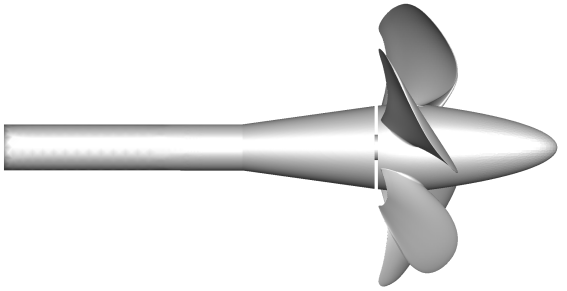
\includegraphics[width=0.4\linewidth]{./fig-material-volume-propeller.png}
    };
    % \begin{scope}[relative to node=image]
    %     \foreach \ratio in {-1,-0.9,...,1}{
    %         \draw[help lines] (-1,\ratio) -- (1,\ratio);
    %         \draw[help lines] (\ratio,-1) -- (\ratio,1);
    %     }
    %     \draw (-1,0) -- (1,0);
    %     \draw (0,-1) -- (0,1);
    % \end{scope}
    \draw[mydarkorange] (\L*1.1,-\Rb*0.8)--(\L*0.9,-\Rb*0.8);
    \draw[mydarkorange] (\L*0.9,-\Rb*0.8) .. controls (\L*0.5,-\Rb*0.8) and (\L*0.4,\Rb*0.8) .. (\L*0.3,\Rb*0.8) to[out=180,in=80] (\L*0.203,\Rb*0.15);
 
    \draw[mydarkorange,-latex] (\L*0.197,\Rb*-0.14) to[out=260,in=60] (\L*0.16,-\Rb*0.7);
    \draw[mydarkorange,-latex] (\L*0.16,\Rb*-0.7) to[out=240,in=-100] (\L*0.05,\Rb*0.7) to[in=190,out=80] (\L*0.07,\Rb*0.85) to[out=10,in=110] (\L*0.09,\Rb*0.7) to[out=-80,in=90] (\L*0.1,\Rb*0.15);
    \draw[mydarkorange] (\L*0.1,-\Rb*0.14) ..controls (\L*0.1,-\Rb) and (\L*0.03,-\Rb) .. (-\L*0.01,-\Rb*0.5);


    %%%% TILAVUUDET

    \coordinate (A) at (0.96*\L,-0.45*\Rb);
    \coordinate (B) at ($(A)+(0.03*\L,0.015*\L)$);
    \coordinate (C) at ($(A)+(0,-0.07*\L)$);
    \coordinate (D) at ($(A)+(-0.07*\L,0)$);
    \coordinate (E) at ($(C)+(0.03*\L,0.03*\L)$);
    \coordinate (F) at ($(B)+(-0.06*\L,0)$);
    \coordinate (G) at ($(C)+(-0.07*\L,0)$);
    \coordinate (H) at ($(E)+(-0.06*\L,0)$);

    \fill (G) circle (1.5pt);
    
    
    \draw[dashed] (E)--(H);
    \draw[dashed] (F)--(H);
    \draw[dashed] (G)--(H);
    \draw[fill=gray!30,fill opacity=0.8,line join=bevel] (A)--(B)--(F)--(D)--cycle;
    \draw[fill=gray!30,fill opacity=0.8,line join=bevel] (A)--(B)--(E)--(C)--cycle;
    \draw[fill=gray!30,fill opacity=0.8,line join=bevel] (A)--(D)--(G)--(C)--cycle;

    \coordinate (AA) at (0.75*\L,-0.34*\Rb);
    \coordinate (BB) at ($(AA)+(0.04*\L,0.02*\L)$);
    \coordinate (CC) at ($(AA)+(-0.02*\L,-0.07*\L)$);
    \coordinate (DD) at ($(AA)+(-0.06*\L,0.02*\L)$);
    \coordinate (EE) at ($(CC)+(0.04*\L,0.03*\L)$);
    \coordinate (FF) at ($(BB)+(-0.05*\L,0.02*\L)$);
    \coordinate (GG) at ($(AA)+(-0.07*\L,-0.054*\L)$);
    \coordinate (HH) at ($(EE)+(-0.05*\L,0.015*\L)$);

    \draw[dashed] (EE) to[bend left=5](HH);
    \draw[dashed] (FF) to[bend right=10] (HH);
    \draw[dashed] (GG) to[bend left=20] (HH);
    \draw[fill=gray!30,fill opacity=0.8,line join=bevel] (AA) to[bend left=20] (BB) to[bend left=20] (FF) to[bend right=20] (DD) to[bend right=20] cycle;
    \draw[fill=gray!30,fill opacity=0.8,line join=bevel] (AA) to[bend left=20] (BB) to[bend right=20] (EE) to[bend right=20](CC) to[bend left=20] cycle;
    \draw[fill=gray!30,fill opacity=0.8,line join=bevel] (AA) to[bend left=20](DD) to[bend right=20] (GG) to[bend right=2] (CC) to[bend left=20] cycle;

    %%%%%%%%%%%%%%%%%%%%%%%%%%%%%%%%%

    

    \draw[latex-,shorten <=3pt] (FF) to[bend right=10] ++(0.03*\L,0.1*\L) node[anchor=south] {$V(t_1)$};

    
    %\draw[latex-,shorten <=3pt] (G) to[bend right=20] ++(0.05*\L,-0.08*\L) node[anchor=north] {$\bm{x}(t_0)$};
    
    \draw[latex-,shorten <=3pt] (F) to[bend right=10] ++(0.03*\L,0.1*\L) node[anchor=south] {$V(t_0)$};

    
    %\draw[latex-,shorten <=3pt] (GG) to[bend right=20] ++(0.07*\L,-0.08*\L) node[anchor=north] {$\bm{x}(t_1)$};

    \draw[-latex,thick,mydarkblue] (GG)-- ++(159:0.06*\L);
    \fill[mydarkred] (GG) circle (1.5pt);
    \node[below right =-0.26cm and -0.67cm of GG,rotate=-14] (TT) {$\begin{aligned}
        %&{\color{mydarkred}\bm{x}}(t_1)\\
        &{\color{mydarkblue}\bm{v}}({\color{mydarkred}\bm{x}}(t_1),t_1)
    \end{aligned}$};

    \draw[-latex,thick,mydarkblue] (G)-- ++(180:0.06*\L);
    \fill[mydarkred] (G) circle (1.5pt);
    \node[below right =-0.1cm and -0.7cm of G] (T) {$\begin{aligned}
        %&{\color{mydarkred}\bm{x}}(t_0)\\
        &{\color{mydarkblue}\bm{v}}({\color{mydarkred}\bm{x}}(t_0),t_0)
    \end{aligned}$};
    
    
\end{tikzpicture}
\end{document}
